\documentclass[11pt,a4paper]{article}

\usepackage[utf8]{inputenc}
\usepackage[T1]{fontenc}
\usepackage{lmodern}
\usepackage[margin=0.82in]{geometry}
\usepackage[table]{xcolor}
\usepackage{array}
\usepackage{tabularx}
\usepackage{booktabs}
\usepackage{enumitem}
\usepackage{titlesec}
\usepackage{fancyhdr}
\usepackage{lastpage}
\usepackage{hyperref}
\usepackage{tikz}

\definecolor{TextInk}{HTML}{233142}
\definecolor{HeadingBlue}{HTML}{1D3557}
\definecolor{AccentTeal}{HTML}{2A7F92}
\definecolor{AccentGold}{HTML}{C58B4E}
\definecolor{RuleGray}{HTML}{D6E0E5}
\definecolor{TableStripe}{HTML}{F3F8FA}
\definecolor{SoftTint}{HTML}{F7F4EE}
\definecolor{SoftBlue}{HTML}{EEF6F8}
\definecolor{SoftGreen}{HTML}{EEF7F0}
\definecolor{SoftRed}{HTML}{FBF0EF}

\hypersetup{
  colorlinks=true,
  linkcolor=HeadingBlue,
  urlcolor=AccentTeal,
  pdftitle={IB Geography SL Study Pack - 2026-04-28},
  pdfauthor={IB Geography SL Preparation}
}

\color{TextInk}
\setlength{\parskip}{0.52em}
\setlength{\parindent}{0pt}
\setlength{\tabcolsep}{6pt}
\renewcommand{\arraystretch}{1.22}
\setlist[itemize]{leftmargin=1.35em,itemsep=3pt,topsep=4pt}
\setlist[enumerate]{leftmargin=1.5em,itemsep=3pt,topsep=4pt}

\newcolumntype{Y}{>{\raggedright\arraybackslash}X}
\newcolumntype{L}[1]{>{\raggedright\arraybackslash}p{#1}}

\titleformat{\section}
  {\normalfont\huge\sffamily\bfseries\color{HeadingBlue}}
  {}{0pt}{}
  [\vspace{0.15em}{\color{AccentGold}\titlerule[1pt]}]

\titleformat{\subsection}
  {\normalfont\Large\sffamily\bfseries\color{AccentTeal}}
  {}{0pt}{}

\titleformat{\subsubsection}
  {\normalfont\large\sffamily\bfseries\color{HeadingBlue}}
  {}{0pt}{}

\titlespacing*{\section}{0pt}{1.4em}{0.65em}
\titlespacing*{\subsection}{0pt}{1.0em}{0.35em}
\titlespacing*{\subsubsection}{0pt}{0.8em}{0.25em}

\pagestyle{fancy}
\setlength{\headheight}{14pt}
\fancyhf{}
\fancyhead[L]{\sffamily\color{AccentTeal}Tue 2026-04-28}
\fancyhead[R]{\sffamily\color{HeadingBlue}IB Geography SL}
\fancyfoot[C]{\sffamily\color{HeadingBlue}\thepage\ of \pageref{LastPage}}
\renewcommand{\headrulewidth}{0.4pt}
\renewcommand{\footrulewidth}{0pt}

\newcommand{\term}[1]{\textcolor{HeadingBlue}{\textbf{#1}}}
\newcommand{\exam}[1]{\textcolor{AccentTeal}{\textbf{#1}}}
\newcommand{\boxnote}[3]{%
\noindent\colorbox{#1}{%
  \begin{minipage}{0.965\textwidth}
  \sffamily
  \textbf{\textcolor{HeadingBlue}{#2}} #3
  \end{minipage}
}}

\begin{document}

\begin{center}
  {\sffamily\bfseries\color{HeadingBlue}\LARGE IB Geography SL Study Pack}\\[0.25em]
  {\sffamily\bfseries\color{AccentTeal}\Large Tuesday 2026-04-28}\\[0.35em]
  {\sffamily\color{TextInk}Food And Health Processes + Global Resource Consumption And Security}
\end{center}

\vspace{0.5em}

\boxnote{SoftBlue}{How this pack follows the plan.}{The April 28 schedule is a
weekday session. \term{Audio 1} covers \term{Food and health} processes,
patterns, and causes, especially \term{food systems} and \term{disease spread}.
\term{Audio 2} covers \term{Global resource consumption and security},
especially \term{trends} and \term{impacts}. The \term{25 minute} practice
block asks you to read one graph or map and turn it into \term{4--5}
short-response points; use the separate April 28 visual-data workbook for that
timed practice.}

\section{Today's Target}

By the end of this session, you should be able to:

\begin{itemize}
  \item explain how a food system links inputs, production, processing,
  distribution, consumption, waste, policy, and health outcomes
  \item distinguish \term{food availability}, \term{food access},
  \term{food utilization}, and \term{food stability}
  \item explain disease spread through environmental conditions, mobility,
  inequality, healthcare, and governance
  \item describe the main drivers of rising resource consumption
  \item explain how resource security depends on access, affordability,
  reliability, governance, and scale
  \item use the \term{water-energy-food nexus} to show trade-offs
  \item turn a map, graph, or table into concise, evidence-based
  short-response points
\end{itemize}

\subsection{Session Structure}

\rowcolors{2}{TableStripe}{white}
\begin{tabularx}{\textwidth}{L{0.2\textwidth}Y L{0.26\textwidth}}
\toprule
\textbf{Part} & \textbf{Focus} & \textbf{Output} \\
\midrule
Audio 1 & Food systems, food-security dimensions, disease diffusion, and
causal chains & One spoken or written food-health process chain \\
Audio 2 & Resource consumption trends, resource-security impacts, nexus
trade-offs, and stewardship & One spoken or written resource-impact chain \\
25 min practice & Read one visual source and convert it into 4--5 response
points & One marked visual-data response in the workbook \\
\bottomrule
\end{tabularx}
\rowcolors{2}{}{}

\boxnote{SoftTint}{Carry-forward from April 26 and April 27.}{Bring forward
the weakest item from your Food and health error log and yesterday's paragraph
practice. If your weakness was vague causal language, make every answer today
use the chain \term{factor} $\rightarrow$ \term{process} $\rightarrow$
\term{pattern} $\rightarrow$ \term{impact} $\rightarrow$ \term{evaluation}.}

\section{Audio 1 Script}

\subsection{Food And Health: Processes, Patterns, Causes, Food Systems, And Disease Spread}

Read this aloud or listen to it using text-to-speech. Pause at each memory
check and answer without looking back.

\textbf{Minute 0--2: the frame.}
Today the Food and health focus is not just "what are the problems?" The focus
is \term{process}, \term{pattern}, and \term{cause}. A process is how change
happens. A pattern is where the outcome is stronger, weaker, concentrated, or
uneven. A cause is the reason that process begins or continues. In Food and
health, strong answers connect all three.

For example, a weak answer says, "Some people are hungry because they are poor."
A stronger geography answer says, "Low income reduces access to nutritious food
because households cannot always afford enough safe and varied food, even where
food is physically available in shops or markets. This can produce a spatial
pattern of undernutrition in poorer households, rural areas, informal
settlements, or regions affected by conflict or weak transport." That answer is
better because it separates \term{availability} from \term{access}, then links
poverty to a visible pattern.

Four words organize food security: \term{availability}, \term{access},
\term{utilization}, and \term{stability}. Availability asks whether enough food
exists in a place. Access asks whether people can obtain it physically,
socially, and economically. Utilization asks whether food is safe, nutritious,
and usable by the body, which depends on diet quality, health, clean water, and
sanitation. Stability asks whether access can continue over time despite price
shocks, drought, conflict, job loss, or supply disruption.

Add measurement language before you move on. IB questions often start with
indicators, not with long theory. Food can be measured using daily calorie
intake, undernourishment, child stunting, food price, food availability, or a
composite measure such as a hunger index. Health can be measured using life
expectancy, infant mortality, child mortality, morbidity, disease incidence,
prevalence rates, BMI, obesity rates, and access to safe water or healthcare.
Each indicator has a limitation. Calorie intake does not show micronutrient
quality. BMI does not explain income, culture, or exercise. Life expectancy is a
broad outcome but does not reveal the exact cause of poor health. A strong
answer therefore uses indicators as evidence, then explains the process behind
them.

\textbf{Memory check.} Say the four food-security words from memory. Then add
one sentence explaining why food can be available nationally while some
households remain food insecure.

\textbf{Minute 2--5: food systems as chains.}
A \term{food system} is the full chain of actors and processes involved in
feeding people. It includes land, water, seeds, fertilizer, labor, farming,
storage, processing, transport, wholesale, retail, marketing, cooking,
consumption, waste, regulation, and public health. Exam answers often improve
when you stop treating food as a product and start treating it as a system.

Food systems shape health in several ways. First, they affect \term{quantity}.
If production, storage, or transport is weak, less food reaches consumers.
Second, they affect \term{quality}. Processing and retail can improve safety
and shelf life, but they can also encourage diets high in sugar, salt, fats, or
ultra-processed foods. Third, they affect \term{price}. Subsidies, trade,
transport costs, energy costs, and market power can make nutritious food either
affordable or unaffordable. Fourth, they affect \term{risk}. Poor storage,
contaminated water, weak refrigeration, or unsafe preparation can increase
disease risk.

Think of a food-system answer as a chain:
\term{input pressure} $\rightarrow$ \term{production or supply change}
$\rightarrow$ \term{price or access change} $\rightarrow$ \term{diet or health
outcome} $\rightarrow$ \term{uneven impact}. For instance, drought can reduce
crop yields. Lower supply can raise prices. Higher prices can reduce access for
low-income households. Reduced access can increase undernutrition or force
people toward cheaper, less nutritious food. The impact is uneven because wealth,
government support, storage, trade links, and social safety nets vary between
places.

Use the four food-security dimensions as a paragraph builder. If a question
asks why a place is food insecure, start with the dimension most visible in the
source. If crops have failed, begin with \term{availability}. If food is present
but too expensive, begin with \term{access}. If illness, poor sanitation, or
unsafe water prevents people from benefiting from food, begin with
\term{utilization}. If a place is normally secure but becomes insecure during
drought, conflict, price shocks, or supply-chain disruption, begin with
\term{stability}. Then add scale. A country may have enough food nationally but
still contain households with poor access. A household may have enough calories
but poor diet quality. A city may have supermarkets but also food deserts,
informal settlements, or groups priced out of nutritious food. This is why the
best answers do not simply say "more food is needed." They explain which part of
the food-security system is failing.

\textbf{Minute 5--7: patterns and causes in food and health.}
Food and health patterns are uneven at multiple scales. At a global scale, some
countries face high levels of undernutrition while others face high levels of
overnutrition and diet-related non-communicable disease. At a national scale,
one region may have better food access, clinics, clean water, or transport than
another. At a city scale, a high-income district may have supermarkets,
healthcare, refrigeration, and safe recreation space, while a low-income
district may have lower food choice, more pollution, worse housing, and weaker
healthcare access.

The IB phrase for this spatial variation is \term{areal differentiation}. It
means that food systems, health outcomes, disease risk, and access to services
differ from place to place. Use the phrase when you compare regions, urban and
rural areas, income groups, or neighborhoods. For example, one area may have
high food availability but poor utilization because water quality and sanitation
are weak. Another area may have high calorie intake but rising obesity and
diabetes risk because diets are changing. Areal differentiation helps you avoid
flat answers. It pushes you to ask: where is the problem most severe, who is
affected, and why does that place differ from another place?

The causes are never only physical. Climate, soil, water, pests, and disease
matter, but so do income, trade, infrastructure, governance, education, gender,
conflict, market power, cultural preferences, advertising, and healthcare.
That is why a good Food and health answer often uses a double explanation:
\term{environmental conditions} create one pressure, while \term{social and
economic conditions} decide who is most exposed and who can respond.

Now define \term{nutrition transition}. It is the shift from traditional diets
and infectious-disease burdens toward more processed foods, higher sugar and fat
intake, more sedentary lifestyles, and greater risk of non-communicable diseases
such as diabetes and heart disease. This does not mean every place follows the
same path. Poorer groups may still face undernutrition while wealthier or urban
groups face overnutrition. That is called a double burden of malnutrition, and
it is a strong way to explain why one country can contain both hunger and
obesity at the same time.

The studied Food and health anchor in the case-study sheet is \term{TNCs in
Brazil (Nestle)}. Use it carefully. It can help with stakeholder questions
about food systems, processed food, supply chains, marketing, employment, and
access. The evaluative point is that a TNC may widen access and create income
opportunities while also increasing concern about processed-food marketing,
nutrition transition, unequal power, and public-health outcomes.

\textbf{Minute 7--10: disease spread.}
Disease spread is also geographical because it has pathways, barriers, and
uneven vulnerability. Some diseases spread through contaminated water or food.
Some spread through vectors such as mosquitoes. Some spread directly between
people through close contact or respiratory transmission. Some are shaped by
mobility networks such as commuting, migration, tourism, conflict displacement,
and trade.

The key IB word here is \term{diffusion}. Diffusion means spread through space.
For disease, \term{contagious diffusion} means spread through direct or close
contact from person to person or nearby place to nearby place. \term{Relocation
diffusion} happens when infected people move and introduce a disease to a new
area. \term{Hierarchical diffusion} means spread through an ordered network,
such as from a major city or transport hub to smaller places. \term{Expansion
diffusion} means the disease spreads outward while remaining present in the
original area. You do not need every type in every answer, but naming one type
can turn a vague sentence about "spread" into a geographical explanation.

When writing about disease spread, avoid naming a disease and then listing
random factors. Build a route. Use this chain:
\term{environmental or social condition} $\rightarrow$ \term{transmission
route} $\rightarrow$ \term{exposed group} $\rightarrow$ \term{health impact}
$\rightarrow$ \term{response or limitation}. For a water-borne disease pathway,
poor sanitation can contaminate water sources. People using that water for
drinking, cooking, or washing may be exposed. Children, elderly people, and
people with weak healthcare access may be more vulnerable. Health impacts can
include illness, lost school or work time, and sometimes death. Responses can
include water treatment, sanitation infrastructure, public health education,
vaccination where relevant, and rapid treatment, but these depend on funding,
governance, trust, and accessibility.

For a vector-borne pathway, climate and land-use conditions may support the
vector. Standing water, poor drainage, warmer conditions, vegetation change, or
urban growth can create breeding habitats. Human movement can then connect
infected and non-infected places. Healthcare systems can reduce mortality and
spread through testing, treatment, information, and prevention.

Use named disease anchors even if you do not memorize statistics today. For a
water-borne pathway, \term{cholera in Haiti after the 2010 earthquake} is a
useful anchor because damaged sanitation, contaminated water, displacement, and
weak health infrastructure made transmission easier. The exam point is not the
number of cases; it is the chain from infrastructure failure to contaminated
water to vulnerable people to public-health response. For a vector-borne
pathway, \term{dengue in Singapore} is a useful anchor because dense urban
settlement, standing water, mosquito breeding habitats, human movement, and
public-health surveillance all shape risk. Singapore also shows that wealth and
governance do not remove disease risk completely; they change the capacity to
monitor, control, and respond. Keep direct respiratory spread as a possible
pathway, but for Food and health revision today, give most weight to water-borne
and vector-borne disease because those are more central to this option.

\textbf{Minute 10--12: turning content into exam points.}
For short-response questions, one point should do one job. Do not try to write a
mini-essay in every sentence. A good point usually has four parts: a clear claim,
one piece of evidence or specific vocabulary, a causal link, and a consequence.
For example: "Unequal food access can produce health inequality because
low-income households may rely on cheaper, less nutritious food, increasing risk
of undernutrition or diet-related disease." That is one useful point. It is
compact but complete.

For command terms, match the verb. \exam{Describe} needs a visible pattern or
feature, such as "Region A has higher child undernutrition than Region B."
\exam{Explain} needs a reason and a process, such as "This may happen because
lower income reduces access to varied food and healthcare." \exam{Suggest}
allows a plausible reason from the source and your own knowledge. \exam{Compare}
needs both similarities and differences where possible. \exam{Analyse} breaks
the issue into parts and shows relationships, for example how income, water
quality, disease exposure, and food prices interact. If you are stuck, write one
sentence for evidence, one for process, and one for consequence.

Here is a model short-response point in spoken form. Region A's high child
undernutrition and lower safe-water access suggest that food insecurity is
linked to both access and utilization. Food may be limited or unaffordable, but
poor water and sanitation can also prevent people from using food safely,
increasing disease risk and worsening child health. A limitation is that the
source does not show income, conflict, seasonality, or household distribution,
so the pattern needs further evidence before a full conclusion.

Final self-test. Name one food indicator, one health indicator, one disease
diffusion type, one named disease example, and one stakeholder. Then connect
them in one spoken sentence. For example: "A high child mortality rate may be
linked to water-borne disease such as cholera where contaminated water and weak
sanitation increase exposure, while governments, NGOs, and health services try
to reduce risk through water treatment and public-health response." That single
sentence contains evidence, process, example, stakeholder, and response. This is
the density you want in Paper 1 short responses.

One last recap before you stop. Food and health questions reward precise
relationships: indicator to pattern, pattern to process, process to impact, and
impact to response. If you can say \term{availability}, \term{access},
\term{utilization}, \term{stability}, \term{areal differentiation},
\term{nutrition transition}, and \term{diffusion} without looking, you have the
core vocabulary for today's Food and health focus.

Pause for ten seconds and test retrieval. If any one of those terms feels weak,
say its definition once, then use it in a sentence about either Nestle in Brazil,
cholera in Haiti, dengue in Singapore, or the workbook's food-health graph.
If the sentence includes a place, a process, and an outcome, it is already more
geographical than a list of facts.

End Audio 1 by saying two chains from memory:

\begin{enumerate}
  \item \term{food-system factor} $\rightarrow$ \term{food-security dimension}
  $\rightarrow$ \term{health outcome}
  \item \term{disease condition} $\rightarrow$ \term{transmission route}
  $\rightarrow$ \term{vulnerable group} $\rightarrow$ \term{response}
\end{enumerate}

\subsection{Food And Health Key Terms}

\rowcolors{2}{TableStripe}{white}
\begin{tabularx}{\textwidth}{L{0.24\textwidth}Y Y}
\toprule
\textbf{Term} & \textbf{Core meaning} & \textbf{How to use it in an answer} \\
\midrule
Food security & Reliable access to sufficient, safe, nutritious food for an
active and healthy life & Use the four dimensions: availability, access,
utilization, and stability \\
Food system & The full chain of actors and processes involved in producing,
moving, consuming, and disposing of food & Link production, processing,
transport, retail, diet, waste, and policy \\
Malnutrition & Poor nutrition, including undernutrition, micronutrient
deficiency, and overnutrition & Avoid using it only as a synonym for hunger \\
Nutrition transition & Shift toward processed foods, higher fat/sugar diets,
sedentary lifestyles, and non-communicable disease & Useful for rising incomes,
urbanization, TNCs, advertising, and lifestyle change \\
Disease diffusion & Spread of disease through space and populations & Explain
through routes, mobility, environment, and public health response \\
Vector-borne disease & Disease transmitted by a living carrier such as a
mosquito & Link to climate, standing water, drainage, housing, and healthcare \\
Water-borne disease & Disease transmitted through contaminated water & Link to
sanitation, water treatment, infrastructure, and poverty \\
Stakeholder & Person or organization with an interest in the issue & Use for
farmers, households, governments, TNCs, NGOs, and health organizations \\
\bottomrule
\end{tabularx}
\rowcolors{2}{}{}

\subsection{Food-System Process Chains}

\rowcolors{2}{TableStripe}{white}
\begin{tabularx}{\textwidth}{L{0.18\textwidth}Y Y}
\toprule
\textbf{Starting factor} & \textbf{Process chain} & \textbf{Evaluation angle} \\
\midrule
Drought or crop stress & Lower yields $\rightarrow$ reduced local availability
$\rightarrow$ higher prices $\rightarrow$ poorer households reduce quantity or
quality of diet & Import capacity, storage, aid, and income support decide how
severe the impact becomes \\
Food processing and marketing & Longer shelf life and wider retail reach
$\rightarrow$ greater access to packaged foods $\rightarrow$ possible nutrition
transition & Benefits of access and jobs must be weighed against diet-related
health risks \\
Weak sanitation & Contaminated water or food $\rightarrow$ water-borne disease
exposure $\rightarrow$ illness and missed school/work & Infrastructure and
healthcare reduce risk, but only if poorer groups can access them \\
Conflict or displacement & Farming disruption and unsafe movement $\rightarrow$
loss of income and food access $\rightarrow$ higher disease and malnutrition
risk & Humanitarian aid may reduce immediate harm but not solve political
causes \\
\bottomrule
\end{tabularx}
\rowcolors{2}{}{}

\section{Audio 2 Script}

\subsection{Global Resource Consumption And Security: Trends And Impacts}

Read this aloud or listen to it using text-to-speech. The goal is to connect
resource trends to human impacts, not to memorize isolated facts.

\textbf{Minute 0--2: the resource-security frame.}
The Paper 2 core unit \term{Global resource consumption and security} is about
who uses resources, who controls resources, who lacks secure access, and how
resource systems can be managed. A resource is not secure just because it exists
physically. \term{Resource security} means reliable, safe, affordable, and
acceptable access over time. That includes physical supply, infrastructure,
governance, price, technology, trade, and resilience under stress.

Add the exam-coded term \term{ecological footprint}. An ecological footprint is
an estimate of the biologically productive land and water needed to support a
person, group, or country's consumption and absorb its waste. It is useful
because it turns consumption into a spatial idea. A high-income country may have
a large footprint because its residents use more energy, transport, meat,
manufactured goods, housing space, and imported products. A lower-income country
may have a smaller average footprint but still face severe local resource
insecurity if water, food, energy, or services are unevenly distributed. So do
not treat footprint and security as identical. Footprint asks how much is used;
security asks whether people have reliable access.

Three words organize the unit: \term{demand}, \term{inequality}, and
\term{management}. Demand rises with population growth, urbanization, rising
incomes, industrialization, transport, digital technology, changing diets, and
consumer culture. Inequality appears because high-income groups and high-income
places usually consume far more energy, materials, water, and goods per person
than poorer groups. Management asks how governments, firms, communities, and
individuals respond through conservation, efficiency, substitution, trade,
infrastructure, recycling, circular economy, and stewardship.

Define \term{resource stewardship} clearly. Stewardship means responsible
management of resources for current and future users. It includes conservation,
efficient use, pollution control, fair access, recycling, ecosystem protection,
and long-term governance. Stewardship is more than using less. It asks who makes
decisions, who benefits, who carries costs, and whether a resource system can
continue under stress. In an essay, stewardship is often the bridge between
problem and response: high consumption creates pressure, insecurity creates
uneven impacts, and stewardship is the set of choices that can reduce pressure
or distribute risk more fairly.

\textbf{Memory check.} Define resource security in one sentence, then add the
question: secure for whom, at what scale, and for how long?

\textbf{Minute 2--5: trends in consumption.}
Resource consumption is not rising evenly everywhere. It is shaped by
development pathways. As incomes rise, many households consume more electricity,
transport fuel, meat, packaged goods, electronics, and built space. As cities
grow, demand rises for construction materials, water, sanitation, energy,
transport, and waste management. As economies industrialize, demand rises for
metals, energy, land, water, and manufactured goods. At the same time,
technology can reduce the resource needed per unit of output, but total
consumption may still rise if population, income, and consumer demand grow
faster than efficiency improves.

The trend language matters. Do not only say "more resources are used." Say
\term{what} is increasing, \term{where} it is increasing most, \term{why} it is
increasing, and \term{so what} the impact is. For example: "Urbanization
increases demand for water and energy because dense populations require piped
water, treatment, lighting, transport, cooling, and waste systems. If
infrastructure investment does not keep pace, resource insecurity may appear as
unreliable water supply, high prices, blackouts, or pollution."

The name for the efficiency idea is \term{decoupling}. \term{Relative
decoupling} means resource use or pollution grows more slowly than the economy.
\term{Absolute decoupling} means total resource use or emissions fall while the
economy still grows. This distinction matters because a country can become more
efficient but still increase total consumption if population, income, and demand
rise faster than efficiency improves. A related problem is the rebound effect:
if a technology becomes cheaper or more efficient, people may use more of it,
reducing some of the environmental benefit. In exam language, decoupling lets
you evaluate whether technology is solving resource pressure or only slowing its
growth.

There are also different views on whether resource pressure is manageable. A
\term{Malthusian} view argues that population and consumption can grow faster
than resource supply, creating scarcity, famine, conflict, or environmental
limits. A \term{neo-Malthusian} view updates this by focusing on modern
population growth, overconsumption, pollution, and planetary limits. An
\term{anti-Malthusian} or \term{Boserupian} view argues that scarcity can
stimulate innovation: people develop new farming methods, technologies,
substitutes, trade systems, or efficiency gains. In a strong Paper 2 answer, do
not choose one view automatically. Use evidence. Some places show real scarcity
and unequal access; other places show that technology and governance can reduce
pressure.

Use those perspectives as essay tools. A Malthusian paragraph is useful when
the source shows rising population, rising demand, or physical limits such as
water scarcity. A Boserupian paragraph is useful when the source shows
innovation, substitution, recycling, efficiency, or new governance. The best
answer usually weighs both. It might argue that technology can increase supply
or efficiency, but only if access to capital, education, infrastructure, and
stable governance exists. Where those conditions are weak, scarcity can still
produce severe inequality even if global production is technically high.

\textbf{Minute 5--7: impacts of resource insecurity.}
Resource insecurity creates social, economic, environmental, and political
impacts. Social impacts include poorer health, time lost collecting water or
fuel, unequal access to services, food insecurity, and reduced education or work
opportunities. Economic impacts include higher production costs, lower farm
yields, supply-chain disruption, price volatility, and slower development.
Environmental impacts include over-abstraction of water, habitat loss, soil
degradation, pollution, greenhouse gas emissions, and waste accumulation.
Political impacts include tension over access, pressure on governments, protest,
conflict risk in fragile settings, and debates over fairness.

Be careful with conflict language. Resource scarcity does not automatically
cause conflict. It can intensify existing poverty, weak governance, inequality,
historical tension, or climate stress. A more accurate sentence is: "Resource
insecurity can increase the risk of social or political tension when it combines
with weak governance, inequality, and limited alternatives."

Resource issues can also become geopolitical. \term{Resource nationalism}
happens when states try to control strategic resources, restrict exports, or use
resource ownership to strengthen political power. Energy dependency can shape
foreign policy because importing countries may worry about price shocks,
pipeline routes, sanctions, or supply disruption. Critical minerals for
batteries, electronics, and renewable-energy infrastructure can create new
dependencies even during a low-carbon transition. The point is not to turn every
resource answer into politics, but to remember that resources are controlled by
institutions, companies, states, and trade networks. Security is therefore about
power as well as physical supply.

\textbf{Minute 7--9: water-energy-food nexus.}
The \term{water-energy-food nexus} is one of the most useful tools in this unit.
It means that water, energy, and food systems affect each other. Food production
needs water and energy. Water supply often needs energy for pumping, treatment,
desalination, or transfer. Energy production can need water for cooling,
hydropower, biofuel crops, or extraction. A decision in one area can solve one
problem while creating another.

Use a nexus chain in Paper 2. Large-scale irrigation can raise food production,
but it may increase water abstraction and energy demand for pumping. Hydropower
can improve energy security and reduce fossil-fuel dependence, but it may flood
land, alter river ecosystems, change downstream water flow, or displace people.
Biofuels can diversify energy supply, but they may compete with food crops for
land and water. Desalination can improve water supply, but it can be expensive,
energy-intensive, and difficult for poorer places to afford.

Add \term{virtual water} and embedded resources to this thinking. Virtual water
means the water used to produce a traded good, especially food or manufactured
products. A country importing wheat, meat, cotton, or electronics may also be
importing the water, energy, land, and pollution pressures embedded in those
goods. This helps explain why consumption in one place creates environmental
pressure somewhere else. It also links Resources back to Food and health:
changing diets can increase demand for water-intensive food, while drought or
water scarcity can raise food prices and worsen food access. In a Paper 2
answer, this gives you a cross-unit sentence: resource consumption affects food
security, health, climate vulnerability, trade, and inequality at the same time.

\textbf{Minute 9--11: e-waste and circular economy.}
The student's resource case-study sheet lists \term{China no longer accepting
our e-waste}. Treat this as a resource-security and waste-management example.
When a high-consuming country exports waste, the environmental burden may shift
to another place. If an importing country tightens restrictions on foreign waste
or e-waste, exporting countries must rethink recycling, domestic processing,
product design, and consumption habits. The geographical point is not only that
waste moved. It is that consumption in one place can create pollution, health
risk, labor risk, and governance pressure in another.

This example fits \term{circular economy}. A linear economy follows
\term{take} $\rightarrow$ \term{make} $\rightarrow$ \term{use} $\rightarrow$
\term{dispose}. A circular economy tries to reduce extraction and waste by
repairing, reusing, recycling, designing products to last longer, recovering
materials, and making producers responsible for end-of-life impacts. The
evaluation is that circular strategies can reduce pressure, but they need
collection systems, regulation, consumer behavior change, technical capacity,
and markets for recovered materials.

Add a second management anchor for May 1: \term{Singapore's water stewardship}.
Singapore has limited natural freshwater, so it manages water security through a
diversified strategy: local catchment, imported water, desalination, and
reclaimed water known as NEWater. Use this as a stewardship example because it
shows long-term planning, technology, public trust, pricing, infrastructure, and
risk management. It also gives evaluation. Desalination and advanced treatment
can strengthen water security, but they require energy, investment, technical
capacity, and public acceptance. Imports can improve supply, but they create
dependency. The broader lesson is that resource security can be improved without
having abundant local resources, but only where governance, finance, technology,
and public cooperation are strong.

Now compare the two examples. The e-waste example shows the problem of a linear
consumer economy: high consumption, short product life, export of waste, and
uneven exposure to pollution. Singapore's water example shows a stewardship
response: long-term planning, technology, diversified supply, and public
management. Together, they give you a useful contrast for exam writing. One
case shows how resource use can shift costs onto other people and places. The
other shows how governance can reduce insecurity, although with trade-offs in
energy use, cost, dependency, and technical complexity. That comparison is much
stronger than memorizing either example as a single fact.

\textbf{Minute 11--12: exam habit.}
For visual data today, use a five-point rhythm. First, state the overall trend
or pattern. Second, name the highest or lowest place, group, or category. Third,
make one comparison using the data. Fourth, suggest a likely reason using course
vocabulary. Fifth, state one impact or limitation. This prevents vague
description and helps you turn a graph or map into exam points quickly.

Here is a model resource point in spoken form. If a source shows rising energy
use with urban growth, the overall trend is increasing resource demand as cities
expand. The likely explanation is that urban households, transport systems,
water treatment, cooling, lighting, and industry all require reliable energy.
The impact is that resource security may improve for connected users while
emissions, costs, or blackout risks rise if supply and infrastructure do not
keep pace. A stronger answer would then evaluate stewardship: efficiency,
renewable energy, pricing, public transport, and building design can reduce
pressure, but they require investment and political support.

Final self-test. Define \term{resource security}, \term{ecological footprint},
\term{decoupling}, and \term{stewardship} in one sentence each. Then say which
perspective is more pessimistic, \term{Malthusian} or \term{Boserupian}, and
why. Finally, connect one example to one theory. For e-waste, you might say that
high ecological footprints in consuming societies create waste pressures that
are shifted through trade, so circular-economy stewardship is needed to recover
materials and reduce pollution. For Singapore water, you might say that a
Boserupian view is visible because scarcity has encouraged technological and
governance responses, but those responses still depend on energy, investment,
and political trust. That balanced final sentence is the habit you need in
Paper 2: do not only describe resource pressure; judge how far management can
reduce it, for whom, and with what trade-offs.

Pause for ten seconds and test retrieval. If one term is weak, connect it to a
case immediately: ecological footprint to e-waste, stewardship to Singapore
water, decoupling to efficiency, and Malthusian or Boserupian thinking to the
debate over whether scarcity is a hard limit or a trigger for innovation.
If the sentence includes scale, inequality, and one management trade-off, it is
ready to become a Paper 2 short response.
Say the chain once slowly, then once at exam speed, so the sequence becomes
automatic before you open the visual-data workbook.

End Audio 2 by saying one resource chain from memory:
\term{consumption driver} $\rightarrow$ \term{resource demand} $\rightarrow$
\term{security pressure} $\rightarrow$ \term{impact} $\rightarrow$
\term{management response} $\rightarrow$ \term{trade-off}.

\subsection{Resource Key Terms}

\rowcolors{2}{TableStripe}{white}
\begin{tabularx}{\textwidth}{L{0.24\textwidth}Y Y}
\toprule
\textbf{Term} & \textbf{Core meaning} & \textbf{How to use it in an answer} \\
\midrule
Resource security & Reliable, safe, affordable access to essential resources
over time & Always ask secure for whom, at what scale, and under what stress \\
Resource scarcity & Insufficient resource quantity or quality relative to
demand & Distinguish physical scarcity from economic or political access
problems \\
Consumption & Use of goods, energy, water, land, materials, or services & Link
to income, urbanization, technology, diet, and lifestyle \\
Ecological footprint & Estimate of biologically productive land and water
needed to support consumption and absorb waste & Useful for inequality in
consumption and sustainability \\
Water-energy-food nexus & Interdependence between water, energy, and food
systems & Use to explain trade-offs and unintended consequences \\
Circular economy & System aiming to reduce waste through repair, reuse,
recycling, durable design, and material recovery & Evaluate using cost,
infrastructure, regulation, and behavior change \\
Stewardship & Responsible management of resources for current and future users
& Use for conservation, governance, intergenerational equity, and shared
responsibility \\
Energy transition & Shift from high-carbon energy systems toward lower-carbon
or renewable systems & Evaluate reliability, cost, minerals, jobs,
infrastructure, and fairness \\
\bottomrule
\end{tabularx}
\rowcolors{2}{}{}

\subsection{Resource Trend And Impact Matrix}

\rowcolors{2}{TableStripe}{white}
\begin{tabularx}{\textwidth}{L{0.22\textwidth}Y Y}
\toprule
\textbf{Trend} & \textbf{Likely impact} & \textbf{Management or evaluation point} \\
\midrule
Rising urban population & Higher demand for water, energy, housing materials,
transport, and waste services & Compact planning and efficient infrastructure
can reduce per-person pressure, but investment must keep pace \\
Rising incomes and changing diets & More demand for meat, processed foods,
packaging, refrigeration, transport, and land & Diet change can improve choice
but may increase land, water, energy, and health pressures \\
Industrialization and manufacturing & Greater demand for energy, minerals,
water, and transport networks & Economic benefits can be large, but pollution
and unequal exposure require regulation \\
Digitalization and electronics & More demand for electricity, rare materials,
devices, and e-waste handling & Recycling and product design help, but informal
e-waste processing can harm workers and environments \\
Climate stress & Drought, flood, heat, and supply disruption can weaken water,
food, and energy security & Adaptation depends on storage, trade, efficiency,
governance, and household income \\
\bottomrule
\end{tabularx}
\rowcolors{2}{}{}

\subsection{Nexus Diagram}

\begin{center}
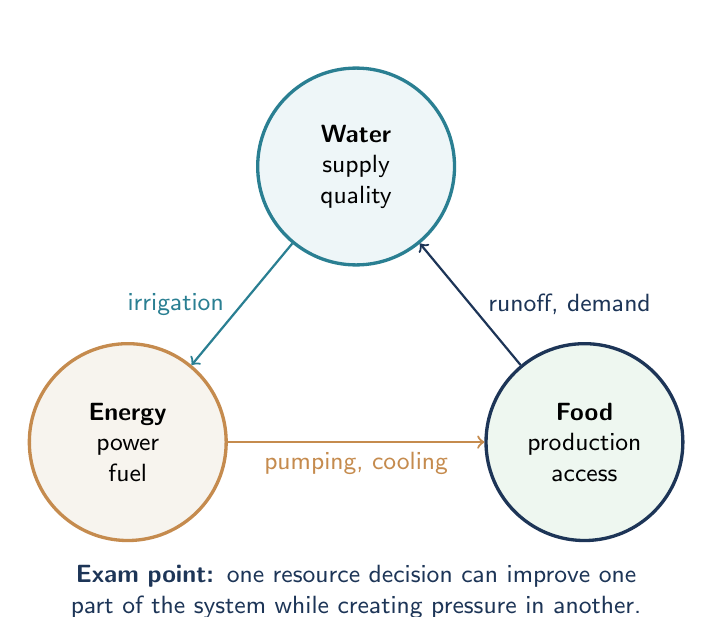
\begin{tikzpicture}[every node/.style={font=\sffamily\small}]
  \node[circle, draw=AccentTeal, very thick, fill=SoftBlue, minimum size=2.5cm,
  align=center] (water) at (0,2.4) {\textbf{Water}\\supply\\quality};
  \node[circle, draw=AccentGold, very thick, fill=SoftTint, minimum size=2.5cm,
  align=center] (energy) at (-2.9,-1.1) {\textbf{Energy}\\power\\fuel};
  \node[circle, draw=HeadingBlue, very thick, fill=SoftGreen, minimum size=2.5cm,
  align=center] (food) at (2.9,-1.1) {\textbf{Food}\\production\\access};
  \draw[->, thick, color=AccentTeal] (water) -- node[left, xshift=-0.1cm]
  {irrigation} (energy);
  \draw[->, thick, color=AccentGold] (energy) -- node[below]
  {pumping, cooling} (food);
  \draw[->, thick, color=HeadingBlue] (food) -- node[right, xshift=0.1cm]
  {runoff, demand} (water);
  \node[align=center, text width=7.6cm, color=HeadingBlue] at (0,-3.0)
  {\textbf{Exam point:} one resource decision can improve one part of the
  system while creating pressure in another.};
\end{tikzpicture}
\end{center}

\section{25-Minute Practice Block}

Use the workbook file
\term{2026-04-28-food-resources-visual-data-workbook.pdf}. The plan asks for
one graph or map, converted into \term{4--5} short-response points.

\subsection{The Five-Point Visual-Data Method}

\rowcolors{2}{TableStripe}{white}
\begin{tabularx}{\textwidth}{L{0.15\textwidth}Y Y}
\toprule
\textbf{Step} & \textbf{Question to ask} & \textbf{Sentence starter} \\
\midrule
1. What & What is the overall pattern or trend? & The main pattern is... \\
2. Where & Where is it highest, lowest, fastest, or most uneven? & The highest
or most affected area is... \\
3. Compare & Which two places, groups, or times differ most? & Compared with...,
... shows... \\
4. Why & Which course process might explain the pattern? & This may be linked
to... because... \\
5. So what & What impact, risk, or management issue follows? & This matters
because... \\
\bottomrule
\end{tabularx}
\rowcolors{2}{}{}

\boxnote{SoftRed}{Important.}{For IB-style visual questions, do not ignore the
source. Use visible evidence first, then add interpretation. If the source is
illustrative rather than official data, treat the values as practice evidence,
not factual statistics to memorize. Do not move invented workbook values into
the May 1 case-study bank as quotable evidence.}

\subsection{End-Of-Day Output}

You are finished with April 28 if you have:

\begin{itemize}
  \item explained food security using availability, access, utilization, and
  stability
  \item written one food-system-to-health process chain
  \item written one disease-spread process chain
  \item defined resource security accurately
  \item explained at least three resource-consumption drivers
  \item used the water-energy-food nexus to show one trade-off
  \item completed one graph or map response with 4--5 marked points
  \item logged one missing case-study detail for Food and health or Resources
\end{itemize}

\boxnote{SoftTint}{May 1 case-study watchlist.}{Today's materials use the two
case anchors currently listed in the student sheet: \term{TNCs in Brazil
(Nestle)} for Food and health and \term{China no longer accepting our e-waste}
for Resources. Before the May 1 case-study bank day, add two missing anchors:
\term{one named disease-spread example} for Food and health and
\term{one second Resources stewardship or management example}. For each, record
place, issue, causes, impacts, response, and one evaluation point.}

\boxnote{SoftGreen}{Carry forward.}{On Wednesday 2026-04-29, the plan moves to
Urban environments essay work plus Population. Bring forward today's visual-data
weakness: if you missed evidence, quote values more directly; if you described
without explaining, add a \term{why} and a \term{so what} sentence.}

\end{document}
